% Schematisch nach Sewing-machine-needles-types.jpg (gemeinfrei).
% Die Spitzen sind zur Unterscheidung vergrößert, nicht maßstäblich.
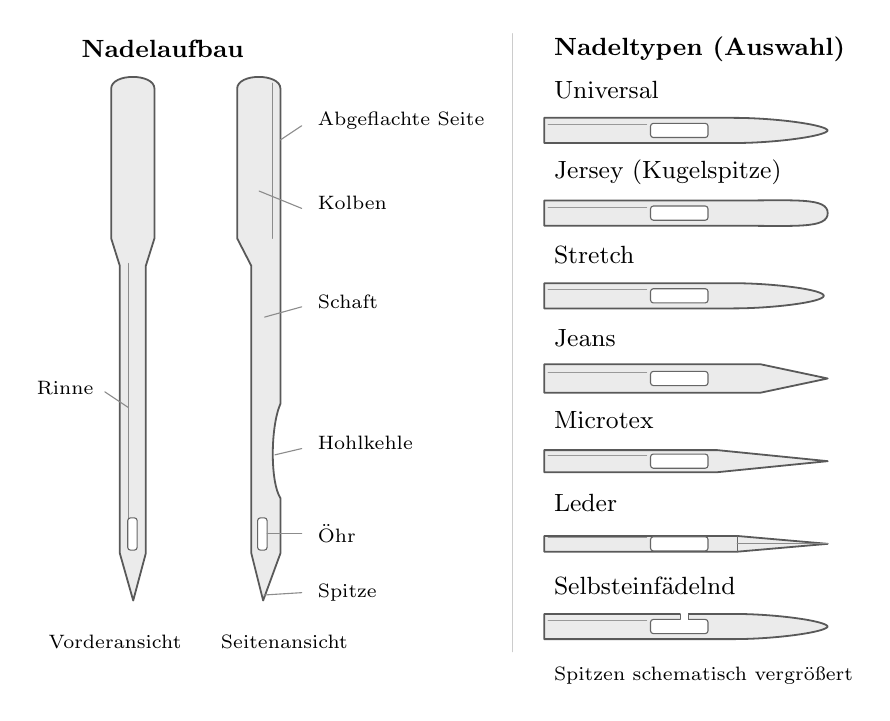
\begin{tikzpicture}[x=1cm,y=1cm,line cap=round,line join=round,
  metall/.style={draw=black!65,fill=black!8,line width=.65pt},
  hinweis/.style={font=\scriptsize,anchor=west},
  typ/.style={font=\small,anchor=west}]
\node[font=\small\bfseries,anchor=west] at (0,7.4){Nadelaufbau};
% Vorder- und Seitenansicht mit dem abgeflachten Kolben.
\path[metall] (.5,6.9) .. controls (.5,7.1) and (1.05,7.1) .. (1.05,6.9)
 -- (1.05,5.0)--(.94,4.65)--(.94,1.0)--(.78,.4)--(.61,1.0)--(.61,4.65)--(.5,5.0)--cycle;
\draw[black!45] (.72,4.68)--(.72,1.05);
\path[draw=black!60,fill=white,rounded corners=1pt] (.71,1.04) rectangle (.83,1.45);
\path[metall] (2.1,6.9) .. controls (2.1,7.1) and (2.65,7.1) .. (2.65,6.9)
 -- (2.65,2.9) .. controls (2.52,2.6) and (2.52,1.9) .. (2.65,1.7)
 -- (2.65,1.0)--(2.43,.4)--(2.28,1.0)--(2.28,4.65)--(2.1,5.0)--cycle;
\draw[black!45] (2.55,6.97)--(2.55,5.0);
\path[draw=black!60,fill=white,rounded corners=1pt] (2.36,1.04) rectangle (2.48,1.45);
% Beschriftungen mit kurzen, getrennten Zeigern.
\node[hinweis] at (3.0,6.5){Abgeflachte Seite}; \draw[black!45] (2.92,6.43)--(2.65,6.25);
\node[hinweis] at (3.0,5.45){Kolben}; \draw[black!45] (2.92,5.38)--(2.38,5.6);
\node[hinweis] at (3.0,4.2){Schaft}; \draw[black!45] (2.92,4.13)--(2.45,4.0);
\node[hinweis] at (3.0,2.4){Hohlkehle}; \draw[black!45] (2.92,2.33)--(2.58,2.25);
\node[hinweis] at (3.0,1.25){Öhr}; \draw[black!45] (2.92,1.25)--(2.48,1.25);
\node[hinweis] at (3.0,.5){Spitze}; \draw[black!45] (2.92,.5)--(2.44,.47);
\node[hinweis,anchor=east] at (.4,3.1){Rinne}; \draw[black!45] (.42,3.05)--(.72,2.85);
\node[font=\scriptsize,align=center] at (.55,-.12){Vorderansicht};
\node[font=\scriptsize,align=center] at (2.7,-.12){Seitenansicht};
% Sieben Spitzenformen, getrennt nach ihrem Typ beschriftet.
\draw[black!20] (5.6,-.25)--(5.6,7.6);
\node[font=\small\bfseries,anchor=west] at (6,7.4){Nadeltypen (Auswahl)};
\foreach \name/\y/\form in {Universal/6.55/1,Jersey (Kugelspitze)/5.5/2,Stretch/4.45/3,Jeans/3.4/4,Microtex/2.35/5,Leder/1.3/6,Selbsteinfädelnd/.25/7}{
 \node[typ] at (6,\y+.34){\name};
 \begin{scope}[shift={(6,\y-.18)}]
 \ifnum\form=2
  \path[metall] (0,-.16)--(2.4,-.16) .. controls (3.2,-.16) and (3.6,-.2) .. (3.6,0)
  .. controls (3.6,.2) and (3.2,.16) .. (2.4,.16)--(0,.16)--cycle;
 \else\ifnum\form=3
  \path[metall] (0,-.16)--(2.4,-.16) .. controls (2.9,-.16) and (3.55,-.08) .. (3.55,0)
  .. controls (3.55,.08) and (2.9,.16) .. (2.4,.16)--(0,.16)--cycle;
 \else\ifnum\form=6
  \path[metall] (0,-.1)--(2.45,-.1)--(3.6,0)--(2.45,.1)--(0,.1)--cycle;
  \draw[black!60] (2.45,-.1)--(2.45,.1); \draw[black!45] (2.45,0)--(3.6,0);
 \else\ifnum\form=4
  \path[metall] (0,-.18)--(2.75,-.18)--(3.6,0)--(2.75,.18)--(0,.18)--cycle;
 \else\ifnum\form=5
  \path[metall] (0,-.14)--(2.2,-.14)--(3.6,0)--(2.2,.14)--(0,.14)--cycle;
 \else
  \path[metall] (0,-.16)--(2.4,-.16) .. controls (2.95,-.16) and (3.58,-.07) .. (3.6,0)
  .. controls (3.58,.07) and (2.95,.16) .. (2.4,.16)--(0,.16)--cycle;
 \fi\fi\fi\fi\fi
 \draw[black!40] (.05,.075)--(1.3,.075);
 \path[draw=black!60,fill=white,rounded corners=1pt] (1.35,-.09) rectangle (2.08,.09);
 \ifnum\form=7
  \path[fill=white] (1.73,.07) rectangle (1.83,.2);
  \draw[black!60] (1.73,.09)--(1.73,.16) (1.83,.09)--(1.83,.16);
 \fi
 \end{scope}
}
\node[font=\scriptsize,anchor=west] at (6,-.55){Spitzen schematisch vergrößert};
\end{tikzpicture}
